%!TEX root = ../thesis.tex

\chapter{Adaptivity}
\label{adp_sec:main}
\section{Introduction}
\paragraph{}
The main objective of this chapter is to introduce a way that can improve the overall mesh quality by refinement automatically and adaptively.
Unnecessary refinement in the region which contributes little to the improvement to the accuracy will be largely prevented.
The expressions related to the eigen-values of the SBFEM formulation representing the quantity of the error in the interpolation are adopted as one of the error indicators, together with the area and other geometric properties of the Scaled Boundary Finite Element.
A machine learning model using the Multilayer Perceptron (MLP) is trained to determine whether a Scaled Boundary Finite Element needs refinement or not based on all these information.

\paragraph{}
The proposed method enhances the SBFEM with quad-tree mesh introduced in Sec.~\ref{qdt_sec:main} and the outstanding features of the method are:
\begin{itemize}
    \item No human effort involvement in mesh refinement
    \item Smart refinement detection
    \item Flexible refinement criteria
\end{itemize}

\paragraph{}
This chapter is organized as follows.
The error indicators used in the proposed method will be introduced first.
After that, a machine learning algorithm that can be trained to determine the necessity of the refinement of a cell based on these indicators.
Furthermore, a triangle merging algorithm is developed to bypass the lack of some error indicators in first order triangle element.\
Finally, the matrix representation of NURBS curves is introduced to improve the computational efficiency and the robustness of the NURBS related calculation.
The accuracy and the convergence properties of the proposed techniques are demonstrated with benchmark problems in the context of linear elasticity, followed by concluding remarks in the last section.


\section{Error indicator}
\label{adap_sec:error_indicator}
\paragraph{}
This section details the proposed error indicators for adaptive scaled boundary finite element analysis.
In comparison with the works in \cite{NME:NME439}, no stress recovery is required.
This reduces the computational effort and leads to an efficient adaptive analysis.
The error estimation is directly invoked from the scaled boundary finite element solutions.

%   ----    %
\subsection{Mesh Size}
\paragraph{}
The area of a subdomain will apparently influences the accuracy of the result.
Generally speaking, a larger subdomain tends to lead to a higher error.
The area of any polygon in Fig.~\ref{adap_fig:ei_polygon} can be calculated as 
%
\begin{equation}
    S = \frac{1}{2}
        \sum_{k=1}
        \left(
            x_k y_{k+1} - x_{k+1} y_k
        \right)
\end{equation}
%
\begin{figure}[h!]
    \centering
    \scalebox{1}{
        \includegraphics{adaptivity/images/adap_ei_polygon.eps}
    }
    \caption{A polygon with $n$ vertexes}
    \label{adap_fig:ei_polygon}
\end{figure}
%
%   ----    %
\subsection{Mesh Quality}
\paragraph{}
Mesh quality is another important factor that influences the accuracy.
In SBFEM, the mesh quality is highly related to the minimal angle formed by the intersecting lines connected to the scaling center and the adjacent polygon vertexes.
An extremely smaller angel as shown in Fig.~\ref{adap_fig:ei_mesh_quality} may raises numerical stability issue and hence decreases the accuracy of the result.

\begin{figure}[h!]
    \begin{subfigure}[b]{0.5\linewidth}
        \centering
        \scalebox{1}{
            \includegraphics{adaptivity/images/adap_ei_mesh_quality_good.eps}
        }
        \caption{Acceptable}
    \end{subfigure}
    \begin{subfigure}[b]{0.5\linewidth}
        \centering
        \scalebox{1}{
            \includegraphics{adaptivity/images/adap_ei_mesh_quality_poor.eps}
        }
        \caption{Unacceptable}
    \end{subfigure}
    \caption[Mesh quality in SBFEM]{Scaling center (
        \tikz[baseline=-0.5ex]\draw[black,fill=black] (0,0) circle (0.7ex);
    ), minimal angle $\alpha$}
    \label{adap_fig:ei_mesh_quality}
\end{figure}
%
%   ----    %
%
\subsection{Eigenvalue in SBFEM}
\paragraph{}
From Eq.~\ref{lr_eq:sbfem_displacement_field} ,the displacement SBFEM can be calculated as
\begin{equation}
    u(\xi) = c_1 \xi ^{-\lambda_1} \phi_u^1
            +c_2 \xi ^{-\lambda_2} \phi_u^2
            +\dots
\label{adap_eq:ei_terms}
\end{equation}
where $\phi_u^i$ stands for the eigenvector corresponding to the $i$th eigenvalue in the eigenvalue matrix $\Lambda^{n}$ in Eq.~\ref{lr_eq:sbfem_eigen_decomp}.
The contribution of each mode is represented by every individual term in Eq.~\ref{adap_eq:ei_terms} \cite{Deeks2002}.
On the other hand, after the displacement solution is calculated on the boundary nodes by Eq.~\ref{lr_eq:sbfem_general_sol_disp} with $\xi=1$, displacement solution in circumferential direction then is interpolated by the help of the $p$-th order shape function $R(\eta)$ in Eq.~\ref{lr_eq:sbfem_displacement_field}.
As a result, terms corresponding to the eigenvalue $\lambda_i \leq p$ can be exactly interpolated by the shape function.
These terms can be regarded as exact.
However, therms corresponding to the eigenvalue $\lambda_i > p$ indicates the shape function is not capable to interpolate the displacement exactly and thus shall be taken as error terms.
Consequently, displacement on the boundary $u(\xi=1)$ can be expressed with exact terms and approximation terms as followed
\begin{equation}
    u_b = u_e (\xi=1) + u_a(\xi=1)
\end{equation}
where the exact terms for the displacement on the boundary can be expressed as
\begin{equation}
    u_e (\xi=1) = \sum c_i \phi_u^i \text{   for all  } \lambda_i \leq p
\end{equation}
and similarly, the approximation terms can be written as
\begin{equation}
    u_a (\xi=1) = \sum c_i \phi_u^i \text{   for all  } \lambda_i > p
\end{equation}
Follow the same logic, nodal forces on the boundary can be expressed As
\begin{equation}
    \begin{aligned}
        q_b &= q_e(\xi=1) + q_a(\xi=1) \\
        q_e(\xi=1) &= \sum c_i \phi_q^i \text{   for all  } \lambda_i \leq p \\
        q_a(\xi=1) &= \sum c_j \phi_q^j \text{   for all  } \lambda_j > p \\
    \end{aligned}
\end{equation}
% energy
The energy can be calculated by the
\begin{equation}
    \begin{aligned}
        U &= \frac{1}{2} u_b^T q_b = U_e + U_a \\
        U_e &= u_e q_e\\
        U_a &= u_e q_a + u_a q_e + u_e q_e
    \end{aligned}
\end{equation}
The relative error for energy can be calculated as $\frac{U_a}{U}$ and the same logic for displacement and stress. 
\paragraph{}
In order to obtain satisfactory solutions within certain accuracy, the contribution of $U_a$ towards $U$ should be minimized and $U_a$ should also be distributed evenly to all cells. This is, in fact, similar to the relative energy norm error used in the literature \cite{NME:NME1620280411}.

\pagebreak

\section{Machine learning}
\paragraph{}
Due to the fact that there are a few error indicators, it could be hard to determine the relationship between them and whether a subdomain need refinement or not.
As a result, specific technique is required in order to search for patterns in the data to find this relationship.
After that a final decision which is a binary classification in this case as each subdomain will be labeled as ``refine'' or ``not refine'' can be made based on the input of the error indicators explained before.
Hence, the discovery of regularities plays a key role in adaptive analysis and an automatic discovery of regularities is usually associated with pattern recognition by the help of algorithms.

%   ----    %
\subsection{Training Set}
\paragraph{}
The training set is determined by numerical examples in fig.~\ref{adap_fig:svm_train_chole} and fig.~\ref{adap_fig:svm_train_cantilever}.
The training data is annotated with whether a subdomain is refined or not and the model can study the data and learn to classify each subdomain based on all four features explained in \ref{adap_error_indicator}.
\begin{figure}[!ht]
    \centering
    \begin{subfigure}[b]{0.5\linewidth}
        \scalebox{0.5}{
            \includegraphics{adaptivity/images/adap_svm_train_chole_0.png}
        }
        \caption{Mesh and displacement field before refinement}
    \end{subfigure}
    \begin{subfigure}[b]{0.5\linewidth}
        \scalebox{0.45}{
            \includegraphics{adaptivity/images/adap_svm_train_chole_1.png}
        }
        \caption{Mesh and displacement field after refinement}
    \end{subfigure}
    \caption{Mesh refinement for square plate with circular hole \cite{Duval2018}}
    \label{adap_fig:svm_train_chole}
\end{figure}

\begin{figure}[!ht]
    \centering
    \begin{subfigure}[b]{0.4\linewidth}
        \scalebox{0.6}{
            \includegraphics{adaptivity/images/adap_svm_train_cantilever_0.png}
        }
    \end{subfigure}
    \begin{subfigure}[b]{0.4\linewidth}
        \scalebox{0.6}{
            \includegraphics{adaptivity/images/adap_svm_train_cantilever_1.png}
        }
    \end{subfigure}\\
    \begin{subfigure}[b]{1\linewidth}
        \centering
        \scalebox{0.7}{
            \includegraphics{adaptivity/images/adap_svm_train_cantilever_2.png}
        }
    \end{subfigure}
    \caption{Mesh refinement of a short cantilever beam \cite{Zienkiewicz2005500}}
    \label{adap_fig:svm_train_cantilever}    
\end{figure}

\paragraph{}
With the same examples, uniform mesh of quadtree is conducted and the same region are marked as refined as shown in fig.~\ref{adap_fig:svm_train_my}.
\begin{figure}[!ht]
    \centering
    \begin{subfigure}[b]{1\linewidth}
        \centering
        \scalebox{0.25}{
            \includegraphics{adaptivity/images/adap_svm_train_my_chole.eps}
        }
    \end{subfigure}
    \begin{subfigure}[b]{0.49\linewidth}
        \scalebox{0.25}{
            \includegraphics{adaptivity/images/adap_svm_train_my_cantilever_0.eps}
        }
    \end{subfigure}
    \begin{subfigure}[b]{0.49\linewidth}
        \scalebox{0.25}{
            \includegraphics{adaptivity/images/adap_svm_train_my_cantilever_1.eps}
        }
    \end{subfigure}
    \caption[Training data for SVM]{Training data for SVM: Cells in black is marked as refined.}
    \label{adap_fig:svm_train_my}
\end{figure}

Criteria taken into consideration are: 
\begin{enumerate}
    \item Ratio of the area of the cell to the total area
    \item Minimal angle formed by the intersecting lines connected by scaling center and adjacent polygon vertexes
    \item Eigenvalue error indicator for displacement
    \item Eigenvalue error indicator for stress
\end{enumerate}

%  ----------------------------------------------------------------------------- %
\subsection{Regularization for MLP}
\paragraph{Bagging}
Bagging is a technique that utilize multiple models in order to increase the accuracy of the prediction \cite{Breiman1996}.
The principle of idea of that is simple: training multiple models separately and let them vote for the prediction.
It is adopted vastly in machine learning.
The reason that model averaging works is that different models will usually not make all the same errors on the test set.
Consider for example a set of k regression models.
Suppose that each model makes an error $\epsilon_i$ on each example, with the errors drawn from a zero-mean multivariate normal distribution with variances $E[\epsilon_i^2]$ = $\nu$ and covariances $E[\epsilon_i \epsilon_j]$=$c$.
Then the error made by the average prediction of all ensemble models is $\frac{1}{k}\sum_i \epsilon_i$.
The expected squared error of the ensemble predictor is 
\begin{equation}
    \begin{aligned}
    E[(\frac{1}{k} \sum_i \epsilon)^2] &=
    \frac{1}{k^2}[
        \sum_i (
            \epsilon_i^2 + \sum_{j\neq i}\epsilon_i \epsilon_j
        )
    ] \\
    &= \frac{1}{k}\nu + \frac{k-1}{k}c
    \end{aligned}
\end{equation}
In the case where the errors are perfectly correlated and $c=\nu$, the mean squared error reduces to $\nu$, so the model averaging does not help at all.
In the case where the errors are perfectly uncorrelated and $c=0$, the expected squared error of the ensemble is only $\frac{1}{k}\nu$.
This means that the expected squared error of the ensemble decreases linearly with the ensemble size.
In other words, on average, the ensemble will perform at least as well as any of its members, and if the members make independent errors, the ensemble will perform significantly better than its members.
\paragraph{}
Different ensemble methods construct the ensemble of the models in different ways.
For example, each member of the ensemble could be formed by training a completely different kind of model using a different algorithm or objective function.
Bagging is a methods that allows the same kind of model, training algorithm and objective function ot be reused serval times.
\paragraph{}
Specifically, bagging involves constructing $k$ different datasets.
Each dataset has the same number of example as the original dataset, but each dataset is constructed by sampling with replacement from the original dataset.
This means that, with high probability, each dataset is missing some of the examples from the original dataset and also contains several duplicate examples(on average around 2/3 of the examples from the original dataset are found in the resulting training set, if it has the same size as original).
Model $i$ is then trained on dataset $i$.
The differences between which examples are included in each dataset result in differences between the trained models.
\paragraph{}
Neural networkds reach a wide enough variety of solution points that they can often benefit from model averaging even if all of the models are trained on the same datase.
Differences in random initialization, random selection of minibatches, differences in hyperparameters, or different outcomes of non-deterministic implementations of neural networks are often enough to cause different members of the ensemble to make partially independent errors.
\paragraph{}
Model averaging is an extremely powerful and reliable method for reducing generalization error.
Machine learning contests are usually won by methods using model averaging over dozens of models.
A recent prominent example is Netflix Grand Price \cite{koren2009}.

\paragraph{Dropout}
Dropout \cite{JMLR:v15:srivastava14a} provides a computationally inexpensive but powerful method of regularizing a broad family of models.
To a first approximation, dropout can be thought of as a method of making bagging practical for ensembles of very many large neural networks.
Bagging involves training multiple models, and evaluating multiple models on each test example.
This seems impractical when each model is a large neural network, since training and evaluating such networks is costly in terms of runtime and memory.
It is common to use ensembles of five to ten neural networks and six models were used to win the ILSVRC \cite{DBLP:journals/corr/SzegedyLJSRAEVR14}.
Dropout provides an inexpensive approximation to training and evaluating a bagged ensemble of exponentially many neural networks.
\paragraph{}
Specifically, dropout trains the ensemble consisting of all sub-networks that can be formed by removing non-output units from an underlying base network.
In most modern neural networks, based on a series of affine transformations and nonlinearities, we can effectively remove a unit from a network by multiplying its output value by zero.
This procedure requires some slight modification for models such as radial basis function networks, which take the difference between the units state and some reference value.
The algorithm of the dropout is presented in terms of multiplication by zero for simplicity, but it can be trivially modified to work with other operations that remove a unit from the network.
\paragraph{}
Recall that to learn with bagging, k different models are defined and k different datasets by sampling from the traning set with replacement are constructed.
After that, each model will be trained based on individual model.
Dropout aims to approximate this process, but with an exponentially large number of neural networks.
Specifically, to train with dropout, we use a minibatch-based learning algorithm that makes small steps, such as stochastic gradient descent.
Each time we load an example into a minibatch, we randomly sample a different binary mask to apply to all of the input and hidden units in the network.
The mask for each unit is sampled independently from all of the others.
The probability of sampling a mask value of one (causing a unit to be included) is hyperparameter fixed before training begins.
It is not a function of the current value of the model parameters or the input example.
Typically, an input unit is included with probability 0.8 and a hidden unit is included with probability 0.5.
We then run forward propagation, back-propagation, and the learning update as usual.
\paragraph{}
More formally, suppose that a mask vector $\mu$ specifies which units to include and $J(\theta,\mu)$ defines the cost of the model defined by parameters $\theta$ and mask $\mu$.
Then dropout training consisits in minimizing $E_\nu J(\theta,\mu)$.
The expectation contains exponentially many terms but we can obtain an unbiased estimate of its gradient by sampling values of $\mu$.
\paragraph{}
Dropput training is not quite the same as bagging training.
In the case of bagging, the models share parameters, with each model inheriting a different subset of parameters from the parent neural network.
This parameter sharing makes it possible to represent an exponential number of models with a tratable amount of memory.
In the case of bagging, each model is trained to convergence on its respective training set.
In the case of dropout, typically most models are not explicitly trained at all.
Usually, the model is large enough that it would be infeasible to sample all possible sub-networks within the lifetime of the universe.
Instead, a tiny fraction of the possible sub-networks are each trained for a single step, and the parameter sharing causes the remaining sub-networks to arrive at good settings of the parameters.
These are the only differences.
Beyond these, dropout follows the bagging algorithms.
For example, the training set encountered by each sub-network is indeed a subset of the original training set sampled with replacement.
To make a prediction, a bagged ensemble must accumulate votes from all of its member.
We refer to this process as inference in this context.
Bagging and dropout has not required that the model be explicitly probabilistic.
It is assumed that the role of the model is to output a probability distribution.
In the case of bagging, each model $i$ produces a probability distribution $p^{(i)}(y|x)$.
The preidiction of the ensemble is given by the arithmetic mean of all these distributions,
\begin{equation}
    \frac{1}{k} \sum_{i=1}^k (y|x)
\end{equation}
In the case of dropout, each sub-model defined by mask vector $\mu$ defines a probability distribution $p(y|x, \mu)$.
The arithmetic mean over all masks is given by
\begin{equation}
    \sum_\mu p(\mu) p(y|x, \mu)
\end{equation}
where $p(\mu)$ is the probability distribution that was used to sample $\mu$ at training time.
Because the sum includes an exponential number of terms, it is intractable to evalute except in cases where the structure of the model permits som form of simplification.
Deep neural networks are not known to permit an tractable simplification.
Instead, we can approximate the inference with sampling, by averaging together the output from many masks.
Even 10-20 masks are often sufficient to obtain good performance.
\paragraph{}
However, there is an even better approach, that allows us to obtain a good approximation to the predictions of the entire ensemble, at the cost of only one forward propagation.
To do so,we change to using the geometric mean rather than the arithmetic mean of the ensemble member's predicted distributions.
Arguments and empirical evidence that the geometric mean performs comparably to the arithmetic mean are presented in the context \cite {WardeFarley2014SelfinformedNN}.
\paragraph{}
The geometric mean of multiple probability distributions is not guaranteed to be a probability distribution.
To guarantee that the result is a probability distribution, we impose the requirement that none of the sub-models assigns probability 0 to any event, and we renormalize the resuliting distribution.
The unnormalized probability distribution defined directly by the geometric mean is given by:
\begin{equation}
    \tilde{p}_{ensemble}(y|x) = 2^d \sqrt{\prod_\mu p(y|x,\mu)}
\end{equation}
where d is the number of units that my be dropped.
A uniform distribution over $\mu$ is used in order to simplify the presentation, but non0uniform distributions are also possible.
To make predictions a re-normalize need to be performed on the ensemble:
\begin{equation}
    p_{ensemble}(y|x) = \frac{
        \tilde{p}_{ensemble}(y|x)
    }{
        \sum_{y^\prime} \tilde{p}_{ensemble}(y^\prime|x)
    }
\end{equation}
A key insight involved in dropout is that we can approximate $p_{ensemble}$ by evaluating $p(y|x)$ in one model: the model with all units but with the weights going out of unit $i$ multiplied by the probability of including unit $i$ \cite{hinton2012}.
The motivation for this modification is to capture the right expected value of the output from that unit.
It is called weight scaling inference rule.
There is not yet any theoretical argument for the accuracy of this approximate inference rule in deep nonlinear networks, but empirically it performs very well.
\paragraph{}
Because we usually use an inclusion probability of $\frac{1}{2}$, the weight scaling rule usually amounts to dividing the weights by 2 at the end of training, and then using the model as usual.
Another way to achieve the same result is to multiply the states of the units by 2 during training.
Either way, the goal is to make sure that the expected total input to a unit at test time is roughly the same as the expected total input to that unit at train time, even though half the unis at train time are missing on average.
\paragraph{}
For many classes of models that do not have nonlinear hidden units, the weight scaling inference rule is exact.
For a simple example, consider a softmax regression classifier with $n$ input variables represented by the vector v:
\begin{equation}
    P(y=y|v)=softmax(W^Tv+b)_y
\end{equation}
We can index into the family of sub-models by element-wise multiplication of the input with a binary vector d:
\begin{equation}
    P(y=y|v;d) = softmax(W^T(d \odot v)+b)_y
\end{equation}





%  ----------------------------------------------------------------------------- %
\subsubsection{Indicator used in adaptivity}
\paragraph{}
The balance of the indicators is highly dependent on classifiers' objective.
Take the spam detector for an example, a false positive can be more dangerous than a false negative as an important e-mail being marked as spam can be a disaster.
While in adaptivity, there may be no favour over either of them.
It is because refine a cell with lower error or leave a cell with higher error unrefined may not produce significant influence on the final result.
As a result, F1 score can be the most important indicator as it takes both recall rate and precision into consideration.


\subsection{Result}
\paragraph{}
All training data are standardized by eq.~\ref{adap_eq:svm_standardized} where $\overline{x}$ and $\sigma$ is the mean and standard deviation of the data.
It makes features in training data have zero means and unit variance.
Cell that need to be refined are labeled as $1$ and the rest are labeled as $0$.
Radial basis function with $\sigma=0.7624$ is adopted as kernel function.
    \begin{equation}
        x^\prime = \frac{x-\overline{x}}{\sigma}
        \label{adap_eq:svm_standardized}
    \end{equation}
Half of the training data (320 out of 640) are used to train the model and the reset are used as a cross validation.
Different class weight is set for testing different performance in regard to all indicators in fig.~\ref{adap_fig:svm_performance_0}.
\begin{figure}[h!]
    \centering
    \scalebox{0.3}{
        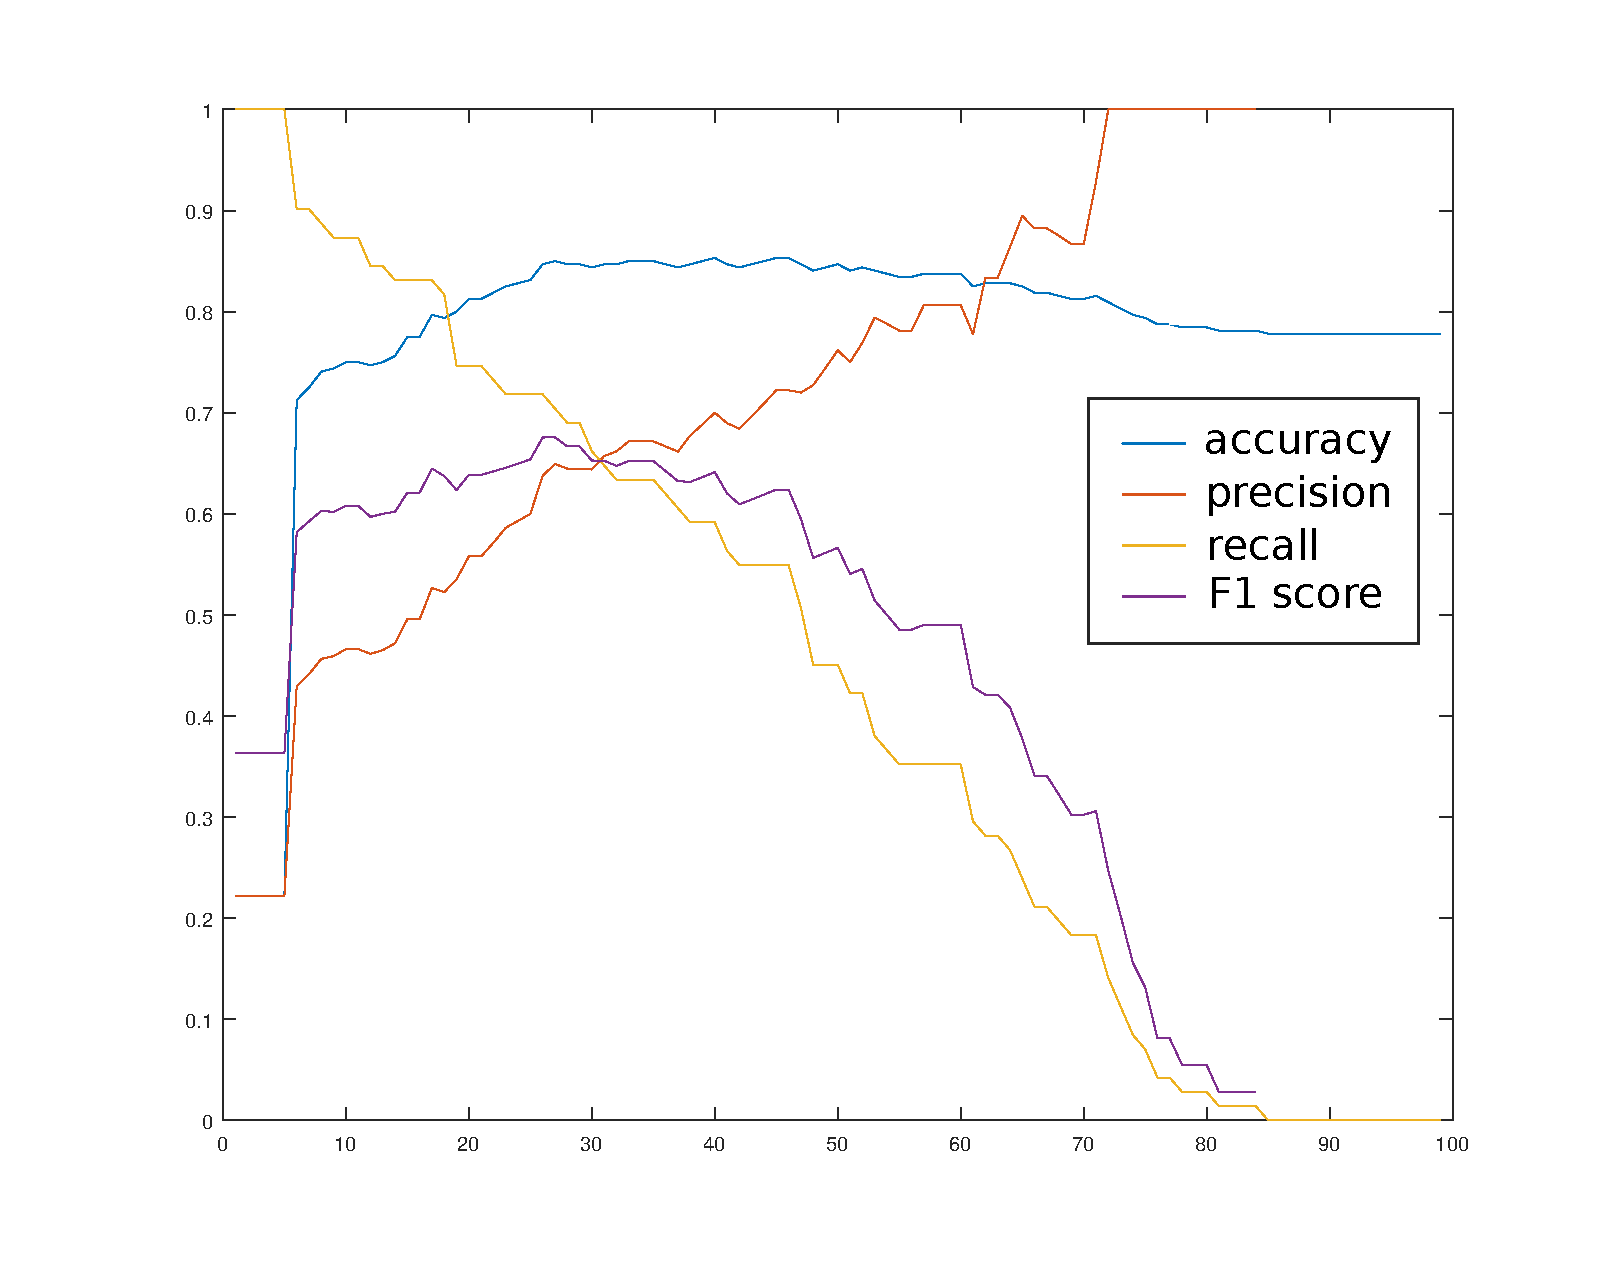
\includegraphics{adaptivity/images/svm_performance_0.eps}
    }
    \caption{Accuracy, precision, recall rate and F1 score vs different class weight}
    \label{adap_fig:svm_performance_0}
\end{figure}
A class weight is a vector that influence the predict directly.
The model will calculate the probability for each classification based on the input and the one with higher probability will be chosen as the result in default situation.
Change class weight to $1:2$ will force the model to choose first class when its probability is more than $66.67\%$ instead of $50\%$.
A class weight of $3:7$ was chosen from fig.~\ref{adap_fig:svm_performance_0} to guarantee a balance between precision and recall rate.
The corresponding result is listed in tab.~\ref{adap_tab:svm_result}.
\begin{table}[h!]
    \centering
    \caption{Result of cross validation}
    \begin{tabular}{cc}
        \toprule
        Accuracy    &   84.38\%    \\
        Precision   &   64.38\%     \\
        Recall rate &   66.20\%     \\
        F1 score    &   65.28\%     \\
        \bottomrule
    \end{tabular}
    \label{adap_tab:svm_result}
\end{table}
%  compare auc
\pagebreak


\section{Merging triangle}
\label{adap_merge_triangle}

\paragraph{}
% why
Due to the property of the SBFEM, first order triangle element will result identical eigenvalues of one.
Under this circumstances, the displacement, nodal forces and energy using eigenvalues failed as the they are always equal to the order of the shape function, one.
As a consequence, the triangular elements shall be merged with their neighbours to form a larger polygon.



\section{Matrix representation of NURBS Curves}
\label{adap_sec_mrep2d}
\subsection{Implicit Matrix Representation}
\paragraph{} 
Matrix representation of a parameterized algebraic curves/surfaces allows a easy way to calculate the intersection between it with another curves and find corresponding parameter based on the given points on the curve/surface. For a algebraic curve $t \in \mathbf{R}^1 \xrightarrow{\phi} \left( \frac{f_1(t)}{f_0(t)}, \frac{f_2(t)}{f_0(t)},\frac{f_3(t)}{f_0(t)} \right) \in \mathbf{R}^3$, $f_0,f_1,f_2$ and $f_3$ are polynomials function in parameter $t$ with degree $\leq p$. The procedure of constructing the matrix representation for NURBS curves and surfaces are explained detail in \cite{Laurent2014}.
\paragraph{}
The aim of this method is to find 4-tuples of polynomials $\left( g_0(t),g_1(t),g_2(t),g_3(t) \right)$ with order $v$ so that
    \begin{equation}
        \sum_{i=0}^3 g_i(t) f_i(t) \equiv 0
        \label{adap_eq_mRep_eq0}
    \end{equation}
who is a vector space and one of its bases can be $$\mathbf{L_j}(t,X,Y,Z) = g_0(t) + Xg_1(t) + Yg_2(t) + Zg_3(t)$$
Since $g$ is also a polynomial based function, it can be expressed in the vector space with a set of bases of $\left\{\psi_1(t), \psi_2(t), \dots, \psi_{m_v}(t) \right\}$ and the bases $\mathbf{L_j}$ can be expressed as
    \begin{equation}
        \begin{aligned}
            \mathbf{L_j} &= \sum^{m_v}_{i=1}\left( \lambda_{0,i}^{(j)} + \lambda_{1,i}^{(j)}X + \lambda_{2,i}^{(j)}Y + \lambda_{3,i}^{(j)}Z\right)\psi_i(t)\\
        & = \sum_{i=1}^{m_v} \Lambda_{i,j}(X,Y,Z)\psi_i(t)
        \end{aligned}
    \end{equation}
Finally, a matrix which represent the mapping of $\phi$ in a $m_v \times r_v$-matrix $\mathbf{M_v}$ with order $v$
    \begin{equation}
        \mathbf{M_v}(\phi) = 
        \begin{bmatrix}
        \Lambda_{1,1} & \Lambda_{1,2} & \dots & \Lambda_{1,r_v} \\ 
        \Lambda_{2,1} & \Lambda_{2,2} & \dots & \Lambda_{2,r_v} \\ 
        \vdots 		  & \vdots 		  &  	  &\vdots			\\
        \Lambda_{m_v,1}&\Lambda_{m_v,2}&\dots &\Lambda_{m_v,r_v}
        \end{bmatrix}
    \end{equation}
\pagebreak



%=====================================================================================================================%
\subsection{Matrix Representation for Rational Bezier Curves}
Rational Bezier curves wit are defined by 
\begin{equation}
	\phi:t\in \mathbf{R}\rightarrow \frac{\sum_{i=0}^pw_i\mathbf{P}_iB_i^p(t) }{\sum_{i=0}^pw_iB_i^p(t)}
\end{equation}
where
    \begin{equation}
        B_i^p(t) = \mathbf{C}_i^dt^i(1-t)^{d-i}
        \label{adap_eq_mrep_bbasis}
    \end{equation}

\paragraph{}
The aim is to have a matrix whose vector is in the form 
    \begin{equation}
        [\alpha] =
        \begin{bmatrix}
            \alpha_{0,0} & \alpha_{0,1}&  \dots&  \alpha_{0,v} & \alpha_{1,0} & \dots & \alpha_{3,v} 
        \end{bmatrix}^T
    \end{equation}
where $g_j(t)$ in the previous section can be expressed as
    \begin{equation}
        g_j(t) = \sum_{i=0}^v \alpha_{j,i}B_i^v(t)
    \end{equation}
Based on eq.~\eqref{adap_eq_mRep_eq0}, it can be concluded that $\mathbf{R}\times\left[\alpha\right]=0$
    \begin{equation}
        \mathbf{R} = 
        \begin{bmatrix}
            B_0^v(t)f_0(t) & \dots & B_v^v(t)f_0(t) & B_0^v(t)f_1(t) & \dots & B_v^v(t)f_3(t)
        \end{bmatrix}
    \end{equation}
By having another set of basis $\mathbf{L_v}$ and the transformation matrix $\mathbf{S}$ so that $\mathbf{L_vS}=\mathbf{R}$ where
    \begin{equation}
        \mathbf{L_v}=
        \begin{bmatrix}
            B_0^{v+d}(t) & B_1^{v+d}(t) & \dots & B_{v+d}^{v+d}(t)
        \end{bmatrix}
    \end{equation}
That leads to
    \begin{equation}
        \begin{bmatrix}
            B_0^{v+d}(t) & B_1^{v+d}(t) & \dots & B_{v+d}^{v+d}(t)
        \end{bmatrix}\times \mathbf{S}\times\left[\alpha\right] = R\times\left[\alpha\right] = 0
    \end{equation}
which indicates $\left[ \alpha\right]$ is in the null space of $\mathbf{S}$;
    \paragraph{}
After substuite $f(t) = \sum_{i=0}^dc_iB_i^d(t)$ into $\mathbf{R}$, the following can be deduced
    \begin{equation}
        B_j^v(t)f(t) =  \sum_{i=0}^dc_iB_i^d(t)B_j^v(t) =\sum_{i=0}^d \frac{\mathbf{C}^v_j\mathbf{C}^d_i}{\mathbf{C}^{d+v}_{i+j}}c_i B_{i+j}^{d+v}(t)
    \end{equation}
which indicates that
    \begin{equation}
        \mathbf{S}_{i+j,j} = \frac{\mathbf{C}^v_j\mathbf{C}^d_i}{\mathbf{C}^{d+v}_{i+j}}c_i
    \end{equation}
Finally, the null space of $\mathbf{S_v}$, $\mathbf{M_v}$ is the matrix representation of the rational bezier curve.
\pagebreak


%=====================================================================================================================%
\subsection{Curve and Curve/Surface Intersection}
The calculation of the intersection is described in detail in \cite{Buse2010} and \cite{Ba2009}. All intersections can be calculated at once by using matrix representation of the algebraic curve/surface.
\paragraph{} 
Given a rational curve/surface $C1$
    \begin{equation}
        \mathbf{P}^1 \xrightarrow{\phi_1} \mathbf{P}^n: (u,v) \rightarrow(f_0,f_1,f_2,f_3)(u,v)
    \end{equation}
the aim of finding the intersection via matrix representation method between it with another ration curve $C2$
    \begin{equation}
        \mathbf{P}^1 \xrightarrow{\phi_2} \mathbf{P}^n: (t) \rightarrow(g_0,g_1,g_2,g_3)(t)
    \end{equation}
is to find
    \begin{equation}
        \mathbf{M}_{v1}(\phi_2(t) = 0
    \end{equation}
which leads to
    \begin{equation}
        \mathbf{M_0}g_0 + \mathbf{M_1}g_1 + \mathbf{M_2}g_2 + \mathbf{M_3}g_3 = 0
        \label{mRep_intec_base}
    \end{equation}
By knowing $g_n$ is a polynomial function with order $p$, eq.~\eqref{mRep_intec_base} can be rearranged as
    \begin{equation}
        \mathbf{M}(t) = \sum_{i=0}^p \mathbf{M_i}t^i
    \end{equation}
After that, the generalized companion $q\times p$-matrices $A,B$ with rank $\rho$are introduced
    \begin{equation}
        A = 
        \begin{bmatrix}
            0		&I 		&\dots 		&\dots 		&0 		\\
            0 		&0 		&I 			&\dots 		&0 		\\
            \vdots 	&\vdots &\vdots 	&\vdots 	&\vdots \\
            0 		&0 		&\dots		&\dots 		&I 		\\
            M_0^t 	&M_1^t 	&\dots 		&\dots 		&M_{d-1}^t
        \end{bmatrix}
    \end{equation}

    \begin{equation}
        B = 
        \begin{bmatrix}
            I 		&0 		&\dots 		&\dots 		&0 		\\
            0 		&I 		&0 			&\dots 		&0 		\\
            \vdots 	&\vdots &\vdots 	&\vdots 	&\vdots \\
            0 		&0 		&\dots 		&I 			&0 		\\
            0 		&0 		&\dots 		&\dots 		&-M_d^t \\		
        \end{bmatrix}
    \end{equation}
Before the eigen values are calculated, the regular part of a non-square pencil of the matrices shall be extracted first which is done by the following step
\paragraph{} 
\textbf{Step 1}
	Transform B into its column echelon form. It is claimed to be performed by adopting LU-decomposition, but I relly don't know how that is accomplished so SVD-decomposition is used in my case
	\begin{equation}
	\begin{aligned}
		B_1 = BV_0 = [\underbrace{B_{1,1}}_{\rho} |\underbrace{0}_{q-\rho}]	\\
		A_1 = AV_0 = [\underbrace{A_{1,1}}_{\rho} |\underbrace{A_{1,2}}_{q-\rho}]
	\end{aligned}
	\end{equation}
\paragraph{} 
\textbf{Step 2}
	Transform $A_{1,2}$ into its row echelon form
	\begin{equation}
		U_1A_{1,2} = 
		\begin{bmatrix}
			\underline{A^\prime_{1,2}}\\
			0
		\end{bmatrix}
	\end{equation}
	where $A^\prime_{1,2}$ is in full row rank.\\
	At the end of step 2, matrix $A$ and $B$ can be represented as
	\begin{equation}
	\begin{aligned}
	A^\prime_1 &=
	\begin{bmatrix}
		A^\prime_{1,1} & A^\prime_{1,2} \\
		\cmidrule(lr){1-2}
		A_2 & 0
	\end{bmatrix}\\
	B^\prime_1 &=
	\begin{bmatrix}
		B^\prime_{1,1} & 0\\
		\cmidrule(lr){1-2}
		B_2 & 0
	\end{bmatrix}
	\end{aligned}
	\end{equation}
where $A^\prime_{1,2}$ has full row rank\\
$
\begin{bmatrix}
\underline{B^\prime_{1,1}}\\
B_2
\end{bmatrix}
$ has full column rank\\
$
\begin{bmatrix}
\underline{B^\prime_{1,1}}\\
B_2
\end{bmatrix}
$ and $B_2$ are in echelon form
\paragraph{}
$A_2$ and $B_2$ will be the new $A$ and $B$ matrices for next iteration until $B$ has full rank. If $B$ has full row rank but not full rank, $A=A^T$, $B=B^T$.
\paragraph{}
After these process, $A$ and $B$ become two square matrices and $B$ is invertible so that the solution for the intersection parameter $t$ can be determined from the eigen value of the matrix $AB^{-1}$
\paragraph{}
This method is proofed to be valid in most of the cases and the line/ NURBS curve/ NURBS surface problem is addressed in our cases. However, the method may fail when the intersection is under the case where nearly tangential geometric conditions happens and return two empty matrices. It is addressed by adding another step after extracting the real part of the $A$ and $B$ if the results are empty matrices\cite{Shen2016}.\\
If the input matrix $A$ and $B$ are not in full row rank or full column rank, it is considered that $C1 \cap C2 = C2$.\\
If the input matrix $A$ and $B$ are in full row rank or full column rank, a rank $m$ square sub-pencil is extracted assuming $A$ and $B$ have a rank of $m$. Then the eigenvalues yield a intersection.


\section{Numerical examples}
% ansys, 12543*2 2nd order 4.92747
% ansys(1st)
% 100*2 - 4.82274
% 361*2 - 4.89143 
% 1369*2 -4.91566
% 5328*2 -4.92411
% err_a1 = abs([4.82274,4.89143,4.91566,4.92411]-4.92747)/4.92747; dof_a1 = [100,361,1369,5328]*2; polyfit(log(dof_a1), log(err_a1),1)


% ansys(2nd)
% 133*2 - 4.88648
% 481*2 - 4.91409
% 1825*2 - 4.92356
% 7105*2 -  4.92685
% err_a2 = abs([4.88648,4.91409,4.92356,4.92685]-4.92747)/4.92747; dof_a2 = [133,481,1825,7105]*2; polyfit(log(dof_a2),log(err_a2),1)

% svm
% 162 - 4.82
% 426 - 4.8945
% 992 - 4.9131
% 1780 - 4.9175
% 2614 - 4.9208
% err = abs([4.82,4.8945,4.9131,4.9175,4.9208] - 4.92747)/4.92747; dof=[162,426,992,1780,2614]; polyfit(log(dof),log(err),1)

% mlp
% 162-4.82
% 496-4.8884
% 1014-4.9090
% 1202-4.9151
% 3146-4.9226
% err = abs([4.82,4.8842,4.9060,4.9180,4.9226] - 4.92747)/4.92747; dof=[162,420,808,1484,3146]; polyfit(log(dof),log(err),1)

\subsection{Short cantilever beam}
\paragraph{}
A two-dimensional short cantilever beam subjected to a uniformly distributed load at the top is examined as shown in Fig.~\ref{adp_fig:ex_cantilever_beam_geo_bc}.
    \begin{figure}[h!]
    \centering
        \scalebox{0.5}{\includegraphics{adaptivity/ex_images/ex_short_cant_geo_bc.eps}}
        \caption{ Short cantilever beam: Geometry and boundary conditions.}
        \label{adp_fig:ex_cantilever_beam_geo_bc}
    \end{figure}

The geometry is: length $L = \SI{1}{\meter} $, height $ D = \SI{1}{\meter} $.
The material properties are: Young’s modulus $ E = \SI{20}{\newton \per \meter^2} $ , Poisson’s ratio $ \nu =0.3 $.
The uniformly distributed load is $w = \SI{10}{\newton \per \meter} $.
Plane stress condition is assumed.

The reference strain energy of \SI{4.02079}{\joule} is determined by the help of the ANSYS.
In the ANSYS, a mesh with $17930$ DOF using 2 \textsuperscript{nd} order plane element $183$ is used to calculate the result.

Due to the fact that the geometry of the cantilever beam can be described by four points and four straight lines, drawing in AutoCAD may not be necessary.
As a result, the input geometry is defined manually.


\paragraph{}
The numerical convergence of the the relative error in the energy norm is shown in Fig.~\ref{adap_fig:ex_short_cantilever_convergence}.
It can be observed that data mining based adaptive SBFEM yields superior convergence rate when compared to the result calculated in ANSYS.

\begin{figure}[h!]
    \centering
    \scalebox{0.5}{
        \includegraphics{adaptivity/ex_images/ex_short_cantilever_conv.eps}
    }
    \caption{the relative error in the energy norm}
    \label{adap_fig:ex_short_cantilever_convergence}
\end{figure}

Corresponding mesh development are plotted in Fig.~\ref{adap_fig:ex_short_cantilever_mesh_develpment} (SBFEM 1\textup{st} order element) and Fig.~\ref{adap_fig:ex_short_cantilever_mesh_develpment_ansys} (ANSYS 9-node quadrilateral element).
Stress contour plotted in ANSYS using 9-node quadrilateral elements (17930 DOFs) are shown in Fig.~\ref{adap_fig:ex_chole_stress_ansys}
\begin{figure}[h!]
\centering
    \begin{subfigure}[b]{0.4\linewidth}
        \centering
        \scalebox{0.25}{
            \includegraphics{adaptivity/ex_images/ex_short_cantilever_mesh_162.eps}
        }
        \caption{Initial mesh (162 DOF)}
    \end{subfigure}
    \begin{subfigure}[b]{0.4\linewidth}
        \centering
        \scalebox{0.25}{
            \includegraphics{adaptivity/ex_images/ex_short_cantilever_mesh_462.eps}
        }
        \caption{1st refinement (462 DOF)}
    \end{subfigure}
    \begin{subfigure}[b]{0.4\linewidth}
        \centering
        \scalebox{0.25}{
            \includegraphics{adaptivity/ex_images/ex_short_cantilever_mesh_992.eps}
        }
        \caption{2nd mesh (992 DOF)}
    \end{subfigure}
    \begin{subfigure}[b]{0.4\linewidth}
        \centering
        \scalebox{0.25}{
            \includegraphics{adaptivity/ex_images/ex_short_cantilever_mesh_1780.eps}
        }
        \caption{3rd refinement (1780 DOF)}
    \end{subfigure}
    \caption{ Short cantilever beam: mesh development (SBFEM)}
    \label{adap_fig:ex_short_cantilever_mesh_develpment}
\end{figure}

\begin{figure}[h!]
    \centering
    \begin{subfigure}[b]{0.48\linewidth}
        \centering
        \scalebox{0.35}{
            \includegraphics{adaptivity/ex_images/ex_short_cantilever_ansys_2_133.png}
        }
        \caption{Initial mesh, 266 DOFs}
    \end{subfigure}
    \begin{subfigure}[b]{0.48\linewidth}
        \centering
        \scalebox{0.35}{
            \includegraphics{adaptivity/ex_images/ex_short_cantilever_ansys_2_481.png}
        }
        \caption{1st refinement, 962 DOFs}
    \end{subfigure}
    \begin{subfigure}[b]{0.48\linewidth}
        \centering
        \scalebox{0.35}{
            \includegraphics{adaptivity/ex_images/ex_short_cantilever_ansys_2_1825.png}
        }
        \caption{2nd refinement, 3650 DOFs}
    \end{subfigure}
    \begin{subfigure}[b]{0.48\linewidth}
        \centering
        \scalebox{0.35}{
            \includegraphics{adaptivity/ex_images/ex_short_cantilever_ansys_2_7105.png}
        }
        \caption{3rd refinement, 14210 DOFs}
    \end{subfigure}
    \caption{Short cantilever beam: mesh development (Ansys)}
    \label{adap_fig:ex_short_cantilever_mesh_develpment_ansys}
\end{figure}

\begin{figure}
    \centering
    \scalebox{0.35}{
        \includegraphics{adaptivity/ex_images/ex_short_cantilever_stress_ansys.png}
    }
    \caption{Von-mises stress contour using 9-node quadrilateral element in ANSYS (17930 DOFs)}
    \label{adap_fig:ex_chole_stress_ansys}
\end{figure}
\pagebreak
%  57205*2 - 11.7733    (ansys 2nd)

% mlp
% 262 - 11.7237
% 940 - 11.7598
% 1408 - 11.7670
% 2176 - 11.7704
% err=abs([11.7237,11.7598,11.7671,11.7704]-11.7733)/11.7733; dof=[262,940,1434,2176]; polyfit(log(dof),log(err),1)

% disperr > 0.005
% 262 - 11.7237
% 664 - 11.7513
% 1112 - 11.7649
% 1316 - 11.7670
% err=abs([11.7237,11.7513,11.7649,11.7670]-11.7733)/11.7733; dof=[262,664,1112,1316]; polyfit(log(dof),log(err),1)

% strerr > 0.01
% 262 - 11.7237
% 860 - 11.7552
% 2792 - 11.7691
% err=abs([11.7237,11.7552,11.7691,]-11.7733)/11.7733; dof=[262,860,2792]; polyfit(log(dof),log(err),1)
% /* cSpell:disable */
% -1 - 282.927
% 382*2  - 274.5638 (32-4/8-3)
% 950*2  - 280.1255 (64-4/8-3)
% 2110*2 - 281.0799 (128-4/15-4)
% 4414*2 - 282.0363 (256-4/15-4)


% mlp
% 530 - 279.8076
% 1554 - 282.0745
% 4208 - 282.5681
% err = abs([279.8076 ,282.0745,282.5681]-282.927)/282.927; dof = [530,1554,4208]; polyfit(log(dof),log(err),1)

% uniform
% 530 - 279.8076
% 1810 - 282.3186
% 6464 - 282.674
% err_un = abs([279.8076 ,282.3186 ,282.674]-282.927)/282.927; dof_un = [530,1810,6464]; polyfit(log(dof_un),log(err_un),1)

% ansys-2nd
% 406*2 -  282.412
% 1144*2 - 282.895
% 4270*2 - 282.923

% 16462*2 -  282.926
% err_a2 = abs([282.412,282.895,282.923]-282.927)/282.927; dof_a2 = [406,1144,4270]*2; polyfit(log(dof_a2),log(err_a2),1)

% ansys-1st
% 185*2 - 275.635    
% 650*2 -  280.006   
% 1227*2 -  281.502 
% 2405*2 - 282.136
% err_a1 = abs([275.635,280.006  ,281.502 ,282.136]-282.927)/282.927; dof_a1 = [185,650,1227,2405]*2; polyfit(log(dof_a1),log(err_a1),1)

% disp > 0.01
% 530 - 279.8076
% 1348 - 281.4530
% 2768 - 282
% 5438 - 282.2
% err_d = abs([279.8076, 281.4530  ,282 ,282.2]-282.927)/282.927; dof_d = [530,1348,2768,5438]; polyfit(log(dof_d),log(err_d),1)

% str > 0.1
% 530 - 279.8076
% 1514 - 281.8970
% 4336 - 282.1295

% err_s = abs([279.8076, 281.8970  ,282.1295 ]-282.927)/282.927; dof_s = [530,1514,4336]; polyfit(log(dof_s),log(err_s),1)


% /* cSpell:enable */

\section{Conclusions}
\paragraph{}
In this chapter, the machine learning algorithm is adopted to develop an extensible and flexible error indicator.
Any other error estimators can be added to the existing framework and their effects can be detected based on the performance indicators in machine learning.
A MLP trained error estimator that concludes expressions related to the eigenvalues of the SBFEM formulation and some key geometric properties of the scaled boundary finite element give a higher convergence rate compared to the uniform refinement.
In order to improve the learning effectiveness of the MLP, regularization methods including bagging and dropout are utilized.
Due to the lack of the eigenvalue error indicator in the first order triangular element, method that eliminates these situation is developed.
A matrix representation of the NURBS curves is presented to achieve a higher efficiency and stability in calculating the intersections between edge\hl{s} of the element and the NURBS curve.
Stress analysis is conducted on 2D linear elasticity problems.